\documentclass[journal,article,submit,oneauthor,pdftex,10pt,a4paper,games]{mdpi} 

\firstpage{1} 
\makeatletter 
\setcounter{page}{\@firstpage} 
\makeatother 
\articlenumber{x}
\doinum{10.3390/------}
\pubvolume{xx}
\pubyear{2017}
\copyrightyear{2017}
\externaleditor{Academic Editor: name}
\history{Received: date; Accepted: date; Published: date}

% import of libraries
\usepackage{algorithm}
\usepackage{algpseudocode}
\usepackage{mathtools}
\usepackage{tikz}
\usepackage{listings}
\usepackage{pgfplots}
\usepackage{color}
\usepackage{subcaption}
\usepackage{mathdots}
\usepackage{hyperref}

% configuration of libraries
\usetikzlibrary{arrows,automata}
\usetikzlibrary{positioning}
\tikzset{
    state/.style={
           rectangle,
           rounded corners,
           draw=black, very thick,
           minimum height=2em,
           inner sep=2pt,
           text centered,
           },
}
\lstset{language=Python}
\pgfplotsset{width=10.5cm,compat=1.8}
\makeatletter

% newcommand for inline equations used in appendices
\newcommand*{\inlineequation}[2][]{
  \begingroup
    \refstepcounter{equation}
    \ifx\\#1\\
    \else
      \label{#1}
    \fi
    \relpenalty=10000
    \binoppenalty=10000
    \ensuremath{
      #2
    }
    ~\@eqnnum
  \endgroup
}
\makeatother



\Title{Non-Markov Stateful Evolutionary Games}
\Author{}
\AuthorNames{}
\address[1]{
 \quad }

\abstract{A new evolutionary game is introduced which incorporates states and actions into the strategies of the organisms of the evolving populations. The game centrally features actions that result in demographic flow between states that may not conserve organism numbers. It is by this feature that the game encapsulate a range of other evolutionary games, and can encode almost very complex interactions between organisms, species and populations.
The game's formalism is expounded and the nature of the game's equilibrium is discussed. This discussion leads to an algorithm for numerically determining the stable equilibrium points which is exemplified in the context of a modified Hawk-Dove game. The game's flexibility for modeling population dynamics is evaluated and compared with other evolutionary games.}
\keyword{Evolutionary stable strategies (ESS); Markov decision evolutionary games (MDEG); Hawk-Dove game; Evolutionary dynamics; Evolutionary Game Theory}

% not sure if I should include these or not?
%\PACS{02.50.Le}
%\MSC{91A22}
%\JEL{C73}


\datasetlicense{CC-BY}
\begin{document}


\section{Introduction}
Biological species are well recognised as being engaged in an fight-for-survival and Evolutionary Game Theory has been used to analyse the strategies in such a fight.
Evolutionary Game Theory encompasses games of different forms, but one of the most standard forms concerns the continuous growth/decay of organism types where the organism types are defined by the strategy they play as they are continuously randomly paired to participate in a simultaneous symmetric two-player game where the expected payoff determines the growth-rate of their strategy.\cite{maynard,maynard2,weibull}

Whereas the sets of actions that actual organisms employ can depend-apon and influence the lifecycles of organisms within an ecosystem, which in turn determines their growth-rate.
These details, such as the stages of the lifecycles of organisms and the web of mutual influences between them, are seldom directly modelled in evolutionary game theory.
Lifecycles are most directly described by matrix models of population dynamics, where the growth-rate of an organism type is naturally given by its population matrix, and where the influences between lifecycle stages are recognised as a potential source of non-linear dynamics and chaotic behaviour \cite{doi:10.1080/10236198.2019.1699916, DEVRIES2020108875, population1}.

Within this paper we consider game-theoretic strategies in the context of lifecycles, and make a contribution by providing a proof that in such games that any search for equilibrium points need only consider pure strategies, and can ignore stochastic combinations of actions - or 'mixed' strategies.
In this way, dynamic points of interest in these complicated games can be discovered and characterised much more directly.

\subsection{Structure}
\begin{itemize}
\item In section \ref{sec:2} we introduce some of the concepts in population matrix models, particularly the concept of \textit{vital rates} and we illustrate how equilibrium population distributions are given by eigenvectors of the population matrix.
\item In section \ref{section:formalism} we give the elements of the game, showing how game-theoretic strategies and vital rates can be brought together to create population matrices for each strategy.
\item In section \ref{sec:equilibria} we give a verbal description of our main result about how equilibrium can be described by pure strategies alone.
\item In section \ref{appendix5} we give the mathematical demonstration of our primary result.
\item And section \ref{sec:conclusion} gives some concluding comments.
\end{itemize}


\section{Related Work}\label{sec:-1}

The formal theory of state has been introduced and considered in the context of population ecology by multiple authors, 
such as by Boling \cite{BOLING1973485} Caswell et.al \cite{nla.cat-vn662318} and Metz \cite{Metz1977}. Particularly Metz \& Diekmann\cite{nla.cat-vn2330051} considered the state of an individual organism (or the `i-state') as the information nessisary to make the response of an organism to its environment determinate, and contrasts this against the population state variable (or 'p-state') characterising the number of individuals in each i-state. 
Where it is possible to consider the population dynamics determined by the p-state, population matrix models have been increasingly employed in ecological studies to model the lifecycles and dynamics of various organisms between states.\cite{doi:10.1111/j.1461-0248.2010.01540.x}
Example models include modelling growth-rate by fecundity across age brackets \cite{leslie}, the dynamics of sexual reproduction and sex ratios \cite{Shyu2018,doi:10.1111/1365-2664.12177} as well as the dynamics of genetic spread and population control measures \cite{DEVRIES2020108875} etc.
In these matrix models, the ratio of population numbers moving between states are called \textit{vital rates}, which directly model the increase or decrease in organism numbers between states.

State also has a history as part of Game Theory literature, particularly the concept of state and actions are most directly modelled in Markov Decision Processes (MDPs) which can bear direct extension to many players in Lloyd Shapley's Stochastic-Games (SG) \cite{shapley53,Solan2015}. Stochastic Games are games where the game itself has a set of possible states or 'positions' (which might be the combination of the states of all players). Within this context each of the individual players have actions which they can execute which jointly determine the likely transitions between the states of the game and the immediate payoffs to each of them.

State has some history in the context of Evolutionary Game Theory, which can be seen in the context of various `evolutionary games on graphs' where the players have the state of belonging to nodes on a grid or graph structure. In these games the players at a node play actions against their nearest neighbours and it can be seen that the structure in these games capture a general sense of position as a state for the players, and this introduces unique and dynamic behaviours.\cite{nowak,spacial2,spacial4}

Another approach of integrating state into Evolutionary Game Theory extends from the works of Eitan Altman et.al \cite{markov2,markov3,markov4,markov5,markov8,markov9} who introduce the Markov-Decision-Evolutionary-Game (MDEG) and variants thereof.
In MDEG games each organism can occupy one of a finite set of states and has actions available to it depending on what state it is in.
The organisms are paired randomly and each of the participants chooses one of their available actions (as determined by their strategy) to execute.
The actions that the organisms execute determine their immediate payoffs and the probable transitions in state that they will make.
The expected sum of payoffs determine the growth-rate of the presence of the strategy in the population, and this then changes the composition of the population in which the random pairings occur.

Our work contrasts against other games, primarily as we model the growth-rate of strategies not in relation to the expected summation of payoffs, but in relation to the equilibrium between states defined by vital rates. This attitude is also reflected in the works of J. M. Cushing \cite{doi:10.1080/10236198.2016.1177522, Cushing2017,doi:10.1080/17513758.2019.1574034} who analyses evolutionary dynamics in population matrix models particularly focusing on bifurcation.

\section{Vital Rates and Population Matrix Models}\label{sec:2}

%It is also worth noting that fitness is not a very simple concept\cite{sep-fitness}
The demographic flow of individuals of a population between states of a lifecycle is sometimes described in ecological-studies by a matrix that is not necessarily Markov.
The simplest example of such matrices are Leslie Matrices used for studying the structure of populations of individuals transitioning between evenly spaced age-states.
Leslie Matrices are square, and they have form \cite{leslie}:

\begin{equation*}
\mathbf{M}=\begin{bmatrix}
    F_0 & F_1 & F_2 & \dots & F_{m-1} & F_m  \\
    P_0 &  0  &  0  & \dots &  0      &  0   \\
     0  & P_1 &  0  & \dots &  0      &  0   \\
     0  &  0  & P_2 & \dots &  0      &  0   \\
    \vdots & \vdots & \vdots & \ddots & \vdots & \vdots \\
     0  &  0  &  0  & \dots  & P_{m-1} &  0   \\
\end{bmatrix}
\end{equation*}
Where $P_i$ represents the probability of and individual in the $i$th age bracket successfully living into the $(i+1)$th age bracket, and $F_i$ is average number of offspring for an individual in $i$th age bracket within the duration of the age bracket.
The positive elements of these matrices identify the `flow' of individuals from one state to another and are called \textit{vital rates}.
For a column vector $\mathbf{n}(t)$ representing the number of individuals in each age-bracket at time $t$, $\mathbf{M}\mathbf{n}(t)$ gives the number of individuals in the population after the duration of one age bracket of time, and $\mathbf{M}^2\mathbf{n}(t)$ the number of individuals after two age brackets, and so on. $$\mathbf{n}(t+1)=\mathbf{M}\mathbf{n}(t)$$
Successive applications eventually yield a steady population profile and a constant exponential growth rate $\lambda$ given by the Euler–Lotka equation, where $\lambda$ is the dominant and only real-positive eigenvalue of the matrix, with the steady population profile $\mathbf{n}$ as its corresponding eigenvector, that is $\mathbf{M}\mathbf{n}=\lambda \mathbf{n}$.

A Leslie matrix is a specific example of a population/projection matrix which projects the growth/decline of a population whose vital rates remain constant.
However, more complicated scenarios exist where the vital rates vary depending on the distribution of the population itself.
For instance, the number of offspring and survival probability to a successive age-state may depend on the density of predators, mates and/or competitors for resources.
In this context the elements of $\mathbf{M}$ may depend on $\mathbf{n}(t)$ in some arbitrary way, which we denote as $\mathbf{M}_{\mathbf{n}(t)}$ and:
$$\mathbf{n}(t+1) = \mathbf{M}_{\mathbf{n}(t)}\mathbf{n}(t)$$
This is the form of a non-linear population matrix model; such models have been shown to yield dynamic behaviours such as non-linear growth, unstable cyclic behaviour and chaos.
Additionally as the matrix $\mathbf{M}$ is non-negative it has a maximum non-negative real eigenvalue $\lambda$ (which might be $1$) and corresponding population vector $\mathbf{n}$
$$\mathbf{M}_{\mathbf{n}}\mathbf{n} = \lambda\mathbf{n}$$
We consider then that the vector $\mathbf{n}$ characterises a potential equilibrium of the population with $\lambda$ its equilibrium growth rate. We now consider how to represent different strategies within the population.


\section{Description of the Game}\label{section:formalism}

Consider an ecosystem of different organisms, where the organisms a set of states and each state has a set of actions which they will execute depending on their strategy. let:

\begin{itemize}
\item	$S$ be indexed finite set of states
%\item   $A$ be the finite set of all actions
\item   $A_s$ be set of actions available organisms in state $s\in S$
\item   $W$ be the set of possible strategies such that for any strategy $w \in W$ that $w_{a,s}$ denotes the probability that an organism with strategy $w$ will execute action $a$ if it is in state $s$.
\item	$P_{s,w}$ is the number of organisms in a state $s\in S$ with strategy $w\in W$; 
\item   $P^*_{s,a} = \sum_{w\in W}P_{s,w}w_{a,s}$ is the number of organisms in a state $s\in S$ which are going to take action $a$.
\item   $T_{s,a}(P^*)$ are vital rates depending\footnote{where $P^*$ is shorthand for the set of all the numbers across $s$ and $a$,  $P^* = \{P^*_{s,a}~|~s\in S,~a\in A_s\}$} on $P^*$, giving the rate of the organism \textit{to} a state $s\in S$ when it executes an action $a\in A_s$.
\end{itemize}



Thus every strategy $w$ has its own population matrix $\mathbf{M}_{P^*}^w$ with components $M^{w}_{i,j}$.%, and population vector $\mathbf{n}^w$.
\begin{equation}\label{eq:transmission_matrix}\mathbf{M}_{P^*}^w = M^{w}_{i,j} = \sum_{a\in A_i}T_{j,a}(P^*) w_{a,i}\end{equation}
And thus the matrix of a strategy $\mathbf{M}_{P^*}^w$ is composed of columns which are weighted by its probability terms $w_{a,s}$,
and it is possible to consider probabilistic mixes of strategies, for instance if strategies $w^1$ and $w^2$ are mixed by a factor $0\le\alpha\le 1$ to form a new strategy $w^\alpha$ whose matrix is then:
\begin{equation}\label{eq:transmission_matrix2}\mathbf{M}_{P^*}^{w^\alpha} = \sum_{a\in A_i}T_{j,a}(P^*) \left(\alpha w^1_{a,i}+(1-\alpha)w^2_{a,i}\right) = \alpha\mathbf{M}_{P^*}^{w^1} + (1-\alpha)\mathbf{M}_{P^*}^{w^2}\end{equation}
In this way one strategy can be considered as a linear combination of other strategies.

\section{Searching for Stable Equilibria}\label{sec:equilibria}

In direct correspondence with common game theory language, it is possible to define basic relationships between the strategies.
Each organism's strategy $w$ encodes the probabilities of what actions it will take across its states.  A strategy is `pure' if these probabilities encode certainty of taking a single action per state otherwise it is `mixed'. Any mixed strategy can be decomposed into a linear combination of pure strategies. And any set of pure strategies defines a span of mixed strategies which can be linearly composed of them.
%The set of pure strategies which could feature in a linear decomposition of a mixed strategy is defined as the `support' of the mixed strategy.

If we define an `equilibrium' as being the condition where all the $\mathbf{M}_{P^*}^w$ population matrices remain constant - and an `equilibrium point' being defined by those matrices.
Then it is necessarily the case that an equilibrium leads to a condition where all the strategies that are significantly present in the population are steadily growing by the same growth-rate in steady-state. For if any organisms of a strategy existed in the population with a lesser steady-state growth-rate then it would proportionally die out, or if any organisms of a strategy existed with a greater steady-state growth-rate then it would lead the others to proportionately die out.

We further define the equilibrium as being `stable' in a similar way to Maynard Smith \cite{maynard, maynard2, weibull}, specifically if it cannot be disturbed from equilibrium by the presence of a small incorporation-of (or `invaded by') any possible `mutant' strategy. We note that this is at-least the case where no `mutant' strategy has a greater steady-state growth-rate in the context of the population.

In the next section \ref{appendix5} there is a demonstration that for any stable equilibrium established with a population of mixed strategies that it is possible to establish the same equilibrium point without the mixed strategies at all.
Informally the reasoning is that: because any mixed strategy is a stochastic mix of pure strategies then it can only perform as well as the best of them. And when it performs equal to the best then they must all perform equally. And in this case there is a combination of the pure strategies which have the same state-action profile $P^*$ as the mixed strategy; the same profile which defines the population matrices and thus the equilibrium point itself.
From these considerations it is thus unnecessary to consider mixed strategies in the search for stable equilibria because every stable equilibria can be established by combinations of pure strategies alone (although there may be zero or multiple such stable equilibria between them).

In our mathematics we assume that all population vectors grow exponentially under stable equilibrium with a common growth-rate equal to a maximum real non-negative eigenvalue (which may be one), and in proportions to a corresponding population matrix eigenvector.
This is a simplifying assumption and there exist possible population matrices where this assumption would be violated (specifically in the context of defective matrices), and in this context, other mathematics would need to be used to assert our conclusions.

\section{That any stable equilibrium point can always be rendered among pure strategies}\label{appendix5}
We consider a strategy's being \textit{replaceable} by other strategies if there exists a possible replacement of one's organisms for the others' in a population such as would not disturb the stable equilibrium point. The equilibrium point is defined by constant matrices $\mathbf{M}_{P^*}^w$, which is preserved at least when $P^*$ remains unchanged.
%Thus a strategy is replaceable at least when it can be replaced by organisms of other strategies such as not to change $P^*$.
If there is a stable equilibrium, each strategy $w$ has population in proportion to an eigenvector $\mathbf{n}^w$ with components $n^w_s$, thus its contribution to $P^*$ (per its definition) is:
$$P_{s,a}w_{a,s} \propto n^w_sw_{a,s}$$
The strategy is replaceable if there is a combination of other strategy's organisms to give this same contribution.

\begin{Definition}\label{def1}
A strategy $\bar{w}$ is \textbf{replaceable at stable equilibrium} by a set of other strategies $W$, if all strategies $w\in W$ are in equilibrium and thus have population matrices with the same maximal real eigenvalue and there exists non-negative corresponding eigenvectors $n^w_s$ and non-negative coefficients $d^w$ such that:
$$\forall a,s~~~~~~~~~~~ n^{\bar{w}}_s\bar{w}_{a,s} = \sum_{w\in W}d^wn^w_sw_{a,s} $$
\end{Definition}

Thus replaceability is a specific relationship between the eigenvectors of different strategy matrices and the weights of the strategies themself (which in turn determine those matrices).
Replaceability has an intuitive transitive property:

\begin{Definition}[Transitive Property of replaceability]\label{def3}
If organisms of strategy $A$ are replaceable by organisms of a set of strategies $B$, and if each of the organisms in the set of strategies in $B$ are replaceable by those of a set of strategies $C$, then organisms of strategy $A$ are also replaceable by those of set of strategies $C$.
\end{Definition}

In light of this we demonstrate that all mixed strategies are replaceable by pure strategies, by showing that every mixed strategy can be iteratively replaced by other strategies that are more `extreme':

\begin{Definition}\label{def2}
A strategy $w$ is \textbf{extreme} with respect to an action $a\in A_{s}$, if $w_{a,s}$ equals zero or one.\\A strategy $w$ is more \textbf{extreme} than another strategy $\bar{w}$ if $w$ is extreme with regards to more actions than $\bar{w}$ is.
\end{Definition}

To make our demonstration we first show that any specific mixed strategy can be decomposed into a linear combination of two strategies more extreme than it, and then we show that the mixed strategy is also replaceable by those two more extreme strategies.

\begin{Lemma}\label{lemma:part1}
Any mixed strategy $\bar{w}$ in stable equilibrium is replaceable by strategies which are more extreme.
\end{Lemma}
\begin{proof}
A mixed strategy $\bar{w}$ is (by definition of mixed) not extreme with regards to some action $\bar{a}\in A_{\bar{s}}$, then we consider two other similar strategies $w^1$ and $w^2$ that are otherwise the same except with re-weighted actions about the $\bar{s}$ state, such as to make them extreme in regards to action $\bar{a}$, ie. that $w^1_{\bar{a},\bar{s}}=1$ and $w^2_{\bar{a},\bar{s}}=0$.
$$ \mathbf{M}_{P^*}^{\bar{w}} = \bar{w}_{\bar{a},\bar{s}}\mathbf{M}_{P^*}^{w^1} + \left(\sum_{a\in A_{\bar{s}}\setminus \{\bar{a}\}} \bar{w}_{a,\bar{s}}\right)\mathbf{M}_{P^*}^{w^2} $$
$$\text{where}\qquad \forall a\in A_{\bar{s}}\setminus \{\bar{a}\},\qquad  w^1_{a,\bar{s}}=0 \quad\text{and}\quad w^2_{a,\bar{s}} = \frac{\bar{w}_{a,\bar{s}}}{\sum_{\hat{a}\in A_{\bar{s}}\setminus \{\bar{a}\}} \bar{w}_{\hat{a},\bar{s}}} $$
We note that if $\bar{w}$ is extreme with regards to any other action $a^*$ then the two other strategies $w^1$ and $w^2$ also extreme with regards to action $a^*$.
Thus any mixed strategy can be considered as a linear combination of two other strategies more extreme than it, all that remains to do is to show that this linear combination is also a replaceable combination aswell.\\
If we consider $\alpha = \bar{w}_{\bar{a},\bar{s}}$ then $\mathbf{M}_{P^*}^{\bar{w}} = \alpha\mathbf{M}_{P^*}^{w^1} + (1-\alpha)\mathbf{M}_{P^*}^{w^2} = \mathbf{M}(\alpha)$ and Theorems \ref{th:2} and \ref{th:3} apply.
Theorem \ref{th:2} informs us that the equilibrium growth rate (the spectral radius of the matrices) of strategies $w^1$ to $\bar{w}$ to $w^2$ is either monotonically increasing or decreasing or otherwise constant.
If it is monotonically increasing/decreasing then either $w^1$ or $w^2$ will have a greater equilibrium growth rate than $\bar{w}$, thus $\bar{w}$ is not part of stable equilibrium creating contradiction; thus $w^1$,$w^2$ and $\bar{w}$ must have the same growth rate.\\
Consequently Theorem \ref{th:3} informs us that the change in eigenvectors are linear, hence $\mathbf{n}^{\bar{w}} = \alpha \mathbf{n}^{w^1} + (1-\alpha)\mathbf{n}^{w^2}$ and that $n^{\bar{w}}_{\bar{s}} = n^{w^1}_{\bar{s}} = n^{w^2}_{\bar{s}}$ and selecting $d^{w^1} = \alpha$ and $d^{w^2} = 1-\alpha$ consequently satisfies definition \ref{def1}.
\end{proof}


\begin{Theorem}\label{the_proof}
Every mixed strategy in stable equilibrium is replaceable by a set of pure strategies 
\end{Theorem}
\begin{proof}
By Lemma \ref{lemma:part1} any mixed strategy can be replaced by other strategies that are more extreme than it, and those strategies (if they are mixed) can then be replaced by strategies which are even more extreme, and so on.
Thus by the transitive property (definition \ref{def3}), every mixed strategy can be replaced by ever increasing sets of strategies which are more extreme, and thus replaced by strategies which are most extreme - ie. pure strategies.
\end{proof}

\section{Conclusion}\label{sec:conclusion}

In this paper we have described a game in the context of non-linear population models, and we have given an equilibrium theorem \ref{the_proof} proving that all equilibria in such games can be found and described by proportions of pure strategies. This theorem's primary utility is that it eliminates the complexity of needing to consider the space of mixed strategies in searching-for and characterising such points of interest.

The elements of the game are simply that there be organisms which move between states in response to the actions and interactions with others,
and the only implicit limitation on such a game is that organisms be sufficiently numerous for their population and their dynamics to be modelled continuously.
Because of this flexibility, it is difficult to understate the potential span of things that could be represented, and therefore the potential applicability of our theorem.
The primary limitation of our theorem is the assumption that equilibrium growth-rates are given by population matrix eigenvalues/vectors (ie. no defective matrices) and thus it is interesting to consider what (if any) populations of things might naturally be described by defective matrices in which our theorem might also fail to hold.




\section{An Example}\label{sec:example}

One of the most famous evolutionary games is that of Hawk-Dove\cite{maynard} which has been extended to multiple states by Eitan Altman et al\cite{markov5, markov3}. A simplified version of Altman's game (as presented in \cite{markov5}) is as follows:
\begin{center}
\fbox{\begin{minipage}{16cm}
Imagine a population of simple organisms that can occupy three distinct distinct States: Young, Aggressive Adult, Passive Adult.
And that the organism's genome encodes a single probability $\gamma$ - that the Young will (if given the opportunity) mature into an Aggressive Adult as opposed to a Passive one.

Imagine that in a distinct unit of time the Young of the population mature into a type of Adult, and also that the Adults die leaving Young offspring.
That a young organism suffers a static probability $C$ of encountering an adult before maturing and if encounters an Aggressive Adult then has a static probability of surviving $D$ and matures into a Passive Adult, otherwise matures into an aggressive Adult or passive adult depending on its genome.

That the Adults in the population of both types have offspring directly dependent on the proportion of Adults that are Aggressive $p$.

Aggressive adults in a population of Passive ones take all resources and have expectation of two offspring, whereas in a population of Aggressive ones expend significant energy fighting for resources and have no offspring. Aggressive adults will have expected offspring $2(1-p)$

Passive adults in a population of Passive adults will generally share resources and save energy by not fighting giving them $1+A$ expected offspring (where $A$ is a static number; $0<A<1$). But in a population of Aggressive ones will loose resources to the Aggressive Adults and have $A$ expected offspring. Passive adults will have expected offspring $1-p+A$
\end{minipage}}
\end{center}

Various observations can be made about this game: \\
Where the population consists entirely of Passive Adults ($p=0$) any organism with $\gamma>0$ might have greater reproductive success and growth rate than the population and thus increase the number of Aggressive Adults.\\
Where the population consists entirely of Aggressive Adults ($p=1$) any organism with $\gamma<1$ might have greater reproductive success and growth rate than the population and thus increase the number of Passive Adults.\\
So there might be an equilibrium in the game\dots?\\ \\
The demographic flow of organisms of between states can be visualized as per Figure \ref{fig:flow}.
\pagebreak


In any-case the game can be formalized as follows:
\begin{itemize}[leftmargin=*,labelsep=4mm]
\item   $K = \{b\}$ A singular species of $b$ird
\item	$S=S_b = \{\mathbf{y},\mathbf{a},\mathbf{p}\}$ are the states of: $\mathbf{y}$oung, $\mathbf{a}$ggressive adult, $\mathbf{p}$assive adult
\item	$A=A_b = \{R_\mathbf{a},R_\mathbf{p},G_\mathbf{a},G_\mathbf{p}\}$, $A_{b,\mathbf{y}}=\{G_\mathbf{a},G_\mathbf{p}\}$, $A_{b,\mathbf{p}}=\{R_\mathbf{p}\}$, $A_{b,\mathbf{a}}=\{R_\mathbf{a}\}$ are actions available to various states: $G_\mathbf{a}$/$G_\mathbf{p}$ is grow into aggressive/passive adult, $R_\mathbf{a}$/$R_\mathbf{p}$ is reproduce aggressively/passively.
\item   All the transmission rates are:\\
\begin{tabular}{cccc}
$T_{b,\mathbf{y},G_\mathbf{a}}(P^*_t)=0$ &
$T_{b,\mathbf{y},G_\mathbf{p}}(P^*_t)=0$ &
$T_{b,\mathbf{y},R_\mathbf{a}}(P^*_t)=2(1-p)$ &
$T_{b,\mathbf{y},R_\mathbf{p}}(P^*_t)=1-p+A$ \\
$T_{b,\mathbf{a},G_\mathbf{a}}(P^*_t)=1-pC$ &
$T_{b,\mathbf{a},G_\mathbf{p}}(P^*_t)=0$ &
$T_{b,\mathbf{a},R_\mathbf{a}}(P^*_t)=0$ &
$T_{b,\mathbf{a},R_\mathbf{p}}(P^*_t)=0$ \\
$T_{b,\mathbf{p},G_\mathbf{a}}(P^*_t)=DpC$ &
$T_{b,\mathbf{p},G_\mathbf{p}}(P^*_t)=DpC+1-pC$ &
$T_{b,\mathbf{p},R_\mathbf{a}}(P^*_t)=0$ &
$T_{b,\mathbf{p},R_\mathbf{p}}(P^*_t)=0$ \\
\end{tabular}
where $A,D,C$ are parameters of the game all between $0$ and $1$, and $p=\frac{P^*_{t,b,\mathbf{a},R_\mathbf{a}}}{P^*_{t,b,\mathbf{a},R_\mathbf{a}}+P^*_{t,b,\mathbf{p},R_\mathbf{p}}}$
\end{itemize}
It is noted that the only state which has multiple actions available to it is $\mathbf{y}$ with $G_\mathbf{a}$ and $G_\mathbf{p}$, and therefore the any strategy $w^b$ is totally specified once $\gamma = w^b_{G_\mathbf{a},\mathbf{y}}$ is specified, thus all strategies of the game can be parameterized by a single number $\gamma$, with $0\le\gamma\le 1$.\\
If the states are indexed in order $\mathbf{y},\mathbf{a},\mathbf{p}$ and the actions are indexed in order $R_\mathbf{a},R_\mathbf{p},G_\mathbf{a},G_\mathbf{p}$ then a strategy $w^b$ where $\gamma = w^b_{G_\mathbf{a},\mathbf{y}}$ has transmission matrix $m_{i,j}$ of the form:
\begin{equation}\label{eq:hd_transmission} m_{i,j} = \begin{bmatrix}
    0 & 2(1-p) & 1-p+A & \\
    \gamma(1-pC) & 0 & 0  & \\
     DpC+(1-\gamma)(1-pC)  & 0 & 0  & \\
\end{bmatrix} \end{equation}
\begin{figure}[]
\begin{center}
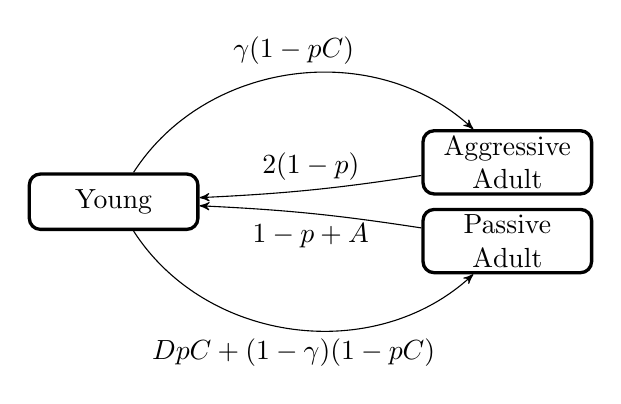
\begin{tikzpicture}[->,>=stealth']

    \node[state,anchor=center,text width=2cm]
        (Y) {Young};
    \node[state,anchor=center,text width=2cm,yshift=0.5cm,right of=Y,node distance=5.0cm]
        (A) {Aggressive\\Adult};
    \node[state,anchor=center,text width=2cm,yshift=-0.5cm,right of=Y,node distance=5.0cm]
        (P) {Passive\\Adult};

    \path (Y) edge[bend left=50]  node[anchor=south,above]{$\gamma(1-pC)$} (A);
    \path (A) edge[bend left=3]   node[anchor=south,above]{$2(1-p)$} (Y);
    \path (P) edge[bend left=-3]   node[anchor=south,below]{$1-p+A$} (Y);
    \path (Y) edge[bend left=-50] node[anchor=south,below]{$DpC+(1-\gamma)(1-pC)$} (P);

\end{tikzpicture}
\end{center}
\caption{A diagram of the demographic flow between states of the example Hawk-Dove game\\$\gamma$ being strategy parameter between $G_\mathbf{a}$ and $G_\mathbf{b}$, $p$ being proportion of Adults that are Aggressive, and $A$,$D$,$C$ being game parameters}
\label{fig:flow}
\end{figure}

We compared the results of the python software (of section \ref{sec:implementation}) on the Hawk-Dove game with those obtained by mathematical analysis (as given in Appendix \ref{appendix3}) and also via stochastic simulation.

The Moran process is a very simple stochastic model of the evolution of finite populations, wherein each 'turn' a random individual is chosen for reproduction proportional to its fitness and a corresponding random individual is chosen for death, the Moran process is generally regarded as a cornerstone technique of stochastic evolutionary game dynamics.\cite{stochastic1}

A Moran process for the above game is programmed (with source-code shown in Appendix \ref{appendix4}) and the results of the Moran process against the python implementation and mathematical analysis are shown in figure \ref{fig:bigfigure}.
The figure shows the value $p$ (the proportion of adults that are aggressive) and the proportion of young ($\%Y$) at equilibrium against the parameter $A$ for fixed $C$ and $D$. The methods of analysis show a strong coincidence in achieving a non-trivial result.

\begin{figure}[]
\begin{center}
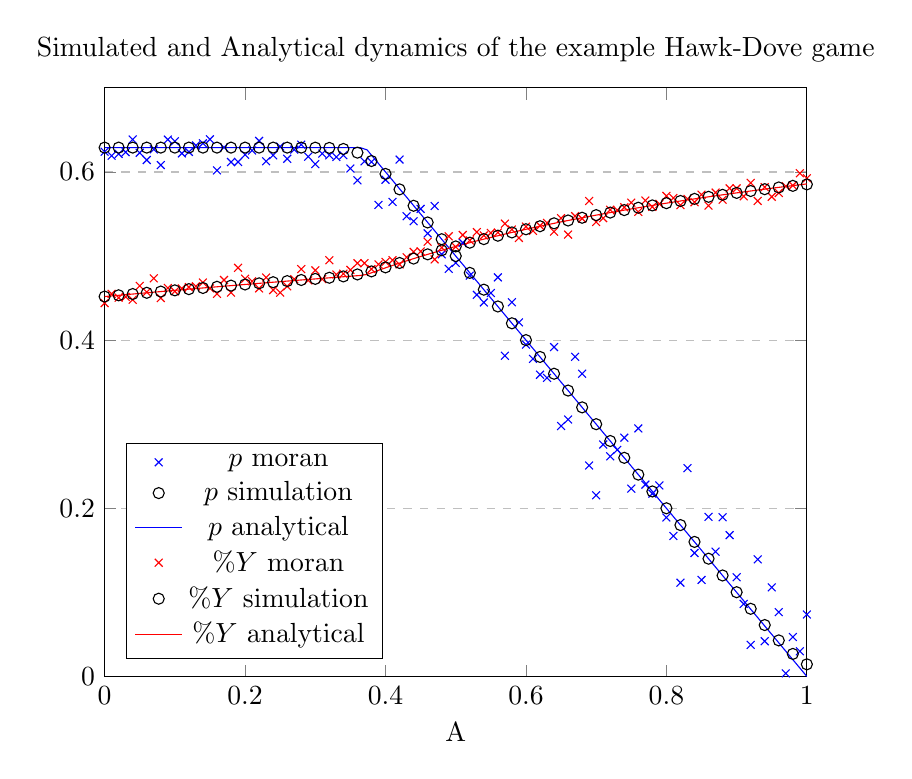
\begin{tikzpicture}
\begin{axis}[
    title={Simulated and Analytical dynamics of the example Hawk-Dove game},
    xlabel={A},
    xmin=0, xmax=1,
    ymin=0, ymax=0.7,
    xtick={0,0.2,0.4,0.6,0.8,1.0},
    ytick={0,0.2,0.4,0.6,0.8,1.0},
    legend pos=south west,
    ymajorgrids=true,
    grid style=dashed,
]
 
\addplot[
    color=blue,
    mark=x,
only marks,
    ]
    coordinates {
    (0.0,0.6241007194244604)(0.01,0.6192660550458715)(0.02,0.62147406733394)(0.03,0.6235186873290793)(0.04,0.6385869565217391)(0.05,0.6227824463118581)(0.06,0.6141804788213628)(0.07,0.6267806267806267)(0.08,0.6081818181818182)(0.09,0.6384758364312267)(0.1,0.6365313653136532)(0.11,0.6220984215413184)(0.12,0.6238361266294227)(0.13,0.6315298507462687)(0.14,0.6340545625587959)(0.15,0.6388115134633241)(0.16,0.6018348623853211)(0.17,0.6291390728476821)(0.18,0.6117755289788408)(0.19,0.6118677042801557)(0.2,0.6204933586337761)(0.21,0.6254716981132076)(0.22,0.6369545032497679)(0.23,0.6127497621313035)(0.24,0.6197964847363552)(0.25,0.6301747930082797)(0.26,0.6156716417910447)(0.27,0.6265402843601896)(0.28,0.6323957322987391)(0.29,0.6181474480151229)(0.3,0.6092843326885881)(0.31,0.6218009478672986)(0.32,0.6198019801980198)(0.33,0.617816091954023)(0.34,0.6199616122840691)(0.35000000000000003,0.6040658276863504)(0.36,0.5899705014749262)(0.37,0.6125860373647984)(0.38,0.612027158098933)(0.39,0.5607843137254902)(0.4,0.5907297830374754)(0.41000000000000003,0.5643564356435643)(0.42,0.6147058823529412)(0.43,0.5473579262213359)(0.44,0.5414141414141415)(0.45,0.5561172901921132)(0.46,0.5269151138716356)(0.47000000000000003,0.5595238095238095)(0.48,0.5020408163265306)(0.49,0.48478488982161594)(0.5,0.4918200408997955)(0.51,0.5157894736842106)(0.52,0.4766355140186916)(0.53,0.45387062566277836)(0.54,0.444794952681388)(0.55,0.4560846560846561)(0.56,0.4745762711864407)(0.5700000000000001,0.38136511375947996)(0.58,0.4450373532550694)(0.59,0.4211076280041797)(0.6,0.3946236559139785)(0.61,0.3776595744680851)(0.62,0.3588362068965517)(0.63,0.3550488599348534)(0.64,0.39171974522292996)(0.65,0.2978021978021978)(0.66,0.3055848261327713)(0.67,0.38011049723756907)(0.68,0.3600439077936334)(0.6900000000000001,0.2508630609896433)(0.7000000000000001,0.21545157780195864)(0.71,0.27582417582417584)(0.72,0.26179775280898876)(0.73,0.26936026936026936)(0.74,0.2839366515837104)(0.75,0.22336769759450173)(0.76,0.29497206703910617)(0.77,0.22811059907834103)(0.78,0.217440543601359)(0.79,0.2271689497716895)(0.8,0.18903150525087514)(0.81,0.16705336426914152)(0.8200000000000001,0.11149032992036405)(0.8300000000000001,0.24768518518518517)(0.84,0.14678899082568808)(0.85,0.11475409836065574)(0.86,0.18977272727272726)(0.87,0.14840989399293286)(0.88,0.18937644341801385)(0.89,0.16805721096543505)(0.9,0.11799761620977355)(0.91,0.08624708624708624)(0.92,0.03753026634382567)(0.93,0.13924050632911392)(0.9400000000000001,0.041866028708133975)(0.9500000000000001,0.10593713620488941)(0.96,0.07647058823529412)(0.97,0.0035971223021582736)(0.98,0.046875)(0.99,0.029887920298879204)(1.0,0.0736196319018405)
    };
\addlegendentry{$p$ moran}
\addplot[
    color=black,
    mark=o,
only marks,
    ]
    coordinates {
(0,0.6289575466)(0.02,0.6289575466)(0.04,0.6289575466)(0.06,0.6289575466)(0.08,0.6289575466)(0.1,0.6289575466)(0.12,0.6289575466)(0.14,0.6289575466)(0.16,0.6289575466)(0.18,0.6289575465)(0.2,0.6289575451)(0.22,0.6289575318)(0.24,0.6289574112)(0.26,0.6289564175)(0.28,0.6289490304)(0.3,0.6289001852)(0.32,0.6286217323)(0.34,0.6273346255)(0.36,0.622964624)(0.38,0.6130200741)(0.4,0.5976515858)(0.42,0.5792825877)(0.44,0.5597835311)(0.46,0.539932344)(0.48,0.5199776121)(0.5,0.4999921004)(0.52,0.4799970362)(0.54,0.4599988331)(0.56,0.4399995329)(0.58,0.4199998251)(0.6,0.3999999577)(0.62,0.3800000258)(0.64,0.360000069)(0.66,0.3400001064)(0.68,0.3200001504)(0.7,0.3000002138)(0.72,0.2800003163)(0.74,0.2600004944)(0.76,0.2400008227)(0.78,0.2200014619)(0.8,0.2000027757)(0.82,0.1800056245)(0.84,0.1600121288)(0.86,0.1400277109)(0.88,0.1200666434)(0.9,0.1001671363)(0.92,0.0804311295)(0.94,0.0611204033)(0.96,0.0428443188)(0.98,0.0267625127)(1,0.0143807301)
    };
\addlegendentry{$p$ simulation}
\addplot [
    domain=0:1, 
    samples=100, 
    color=blue,
    ]
    {min(1-x,(-1*(0.7+1)+sqrt((0.7+1)^2+4*(0.75*0.7-0.7)))/(2*(0.75*0.7-0.7)))};
\addlegendentry{$p$ analytical}

\addplot[
    color=red,
    mark=x,
only marks,
    ]
    coordinates {
    (0.0,0.444)(0.01,0.455)(0.02,0.4505)(0.03,0.4515)(0.04,0.448)(0.05,0.4645)(0.06,0.457)(0.07,0.4735)(0.08,0.45)(0.09,0.462)(0.1,0.458)(0.11,0.4615)(0.12,0.463)(0.13,0.464)(0.14,0.4685)(0.15,0.4615)(0.16,0.455)(0.17,0.4715)(0.18,0.4565)(0.19,0.486)(0.2,0.473)(0.21,0.47)(0.22,0.4615)(0.23,0.4745)(0.24,0.4595)(0.25,0.4565)(0.26,0.464)(0.27,0.4725)(0.28,0.4845)(0.29,0.471)(0.3,0.483)(0.31,0.4725)(0.32,0.495)(0.33,0.478)(0.34,0.479)(0.35000000000000003,0.4835)(0.36,0.4915)(0.37,0.4915)(0.38,0.4845)(0.39,0.49)(0.4,0.493)(0.41000000000000003,0.495)(0.42,0.49)(0.43,0.4985)(0.44,0.505)(0.45,0.5055)(0.46,0.517)(0.47000000000000003,0.496)(0.48,0.51)(0.49,0.5235)(0.5,0.511)(0.51,0.525)(0.52,0.5185)(0.53,0.5285)(0.54,0.5245)(0.55,0.5275)(0.56,0.528)(0.5700000000000001,0.5385)(0.58,0.5315)(0.59,0.5215)(0.6,0.535)(0.61,0.53)(0.62,0.536)(0.63,0.5395)(0.64,0.529)(0.65,0.545)(0.66,0.5255)(0.67,0.5475)(0.68,0.5445)(0.6900000000000001,0.5655)(0.7000000000000001,0.5405)(0.71,0.545)(0.72,0.555)(0.73,0.5545)(0.74,0.558)(0.75,0.5635)(0.76,0.5525)(0.77,0.566)(0.78,0.5585)(0.79,0.562)(0.8,0.5715)(0.81,0.569)(0.8200000000000001,0.5605)(0.8300000000000001,0.568)(0.84,0.564)(0.85,0.573)(0.86,0.56)(0.87,0.5755)(0.88,0.567)(0.89,0.5805)(0.9,0.5805)(0.91,0.571)(0.92,0.587)(0.93,0.5655)(0.9400000000000001,0.582)(0.9500000000000001,0.5705)(0.96,0.575)(0.97,0.583)(0.98,0.584)(0.99,0.5985)(1.0,0.5925)
    };
\addlegendentry{$\%Y$ moran}

\addplot[
    color=black,
    mark=o,
only marks,
    ]
    coordinates {
(0,0.4517891488)(0.02,0.4533007859)(0.04,0.4547950448)(0.06,0.4562723037)(0.08,0.4577329282)(0.1,0.4591772724)(0.12,0.4606056792)(0.14,0.4620184805)(0.16,0.4634159981)(0.18,0.4647985439)(0.2,0.4661664205)(0.22,0.467519924)(0.24,0.4688593629)(0.26,0.4701852059)(0.28,0.4714991067)(0.3,0.4728101081)(0.32,0.4741654624)(0.34,0.4757588605)(0.36,0.4780953866)(0.38,0.4817321369)(0.4,0.4865074548)(0.42,0.4917375503)(0.44,0.4969566765)(0.46,0.501998492)(0.48,0.5068270573)(0.5,0.5114452157)(0.52,0.5158650917)(0.54,0.5201001195)(0.56,0.52416307)(0.58,0.5280656464)(0.6,0.5318184805)(0.62,0.5354312238)(0.64,0.5389126531)(0.66,0.5422707686)(0.68,0.5455128809)(0.7,0.5486456873)(0.72,0.5516753368)(0.74,0.5546074882)(0.76,0.5574473581)(0.78,0.5601997623)(0.8,0.5628691478)(0.82,0.565459611)(0.84,0.567974887)(0.86,0.5704182752)(0.88,0.5727924)(0.9,0.5750985588)(0.92,0.5773350747)(0.94,0.5794935866)(0.96,0.5815525074)(0.98,0.583471595)(1,0.5852028369)
    };
\addlegendentry{$\%Y$ simulation}

\addplot [
    domain=0:1, 
    samples=100, 
    color=red,
    ]
    {max(sqrt(2*x)/(sqrt(2*x)+sqrt(0.7*(1-x)*(0.75-1)+1)), (sqrt(0.75*0.6289575465860742*0.7*(1+0.6289575465860742+x)))/(sqrt(0.75*0.6289575465860742*0.7*(1+0.6289575465860742+x))+1-0.6289575465860742*0.7+0.75*0.6289575465860742*0.7))};
\addlegendentry{$\%Y$ analytical}
 
\end{axis}
\end{tikzpicture}
\caption{Dynamics of the Hawk-Dove game across parameter $A$, with $D = 0.75$ and $C = 0.70$\\ shown are results for $p$ as well as proportion Young $\%Y$ for Moran stochastic simulation, analytical solution, and our software solver's results}
\label{fig:bigfigure}
\end{center}
\end{figure}


\section{Discussion}\label{sec:discussion}

The game (as defined in section \ref{section:formalism}) is designed with broad features to encapsulate a large number of potential applications.
The game's elements consist of there being a population/s of entities that can be described as stateful and stochastically transmit themselves between states based on their present state and the states and actions of others in accordance with a conserved strategy of choosing actions.

It should be quite straightforward that the game's representation encapsulates other evolutionary games:
\newpage
\begin{itemize}[leftmargin=*,labelsep=4mm]
\item   \textbf{Classical evolutionary games} feature a finite set of strategies, each with growth-rates according to the expected payoff against the population of strategies. The rather degenerate analogue in our game, would have a single species with a single state and multiple actions of transmission to that same single state. Each of these actions would correspond to a strategy and would have transmission in proportion to its payoff.
\item   \textbf{Spacial evolutionary games} feature a finite set of strategies across nodes, each with growth-rates according to expected payoff against its neighbors.
The analogue in our game, would consist in modeling each node as a separate species, each with a single state and multiple action of transmission to the single state. Each action would correspond to a strategy at a node and any action's transmission would be in proportion to its payoff against its neighbors.
\end{itemize}
Furthermore we observed (although not yet proven) that MDEG games are also encapsulated: 
\begin{itemize}[leftmargin=*,labelsep=4mm]
\item   \textbf{MDEG games} seem to be closely analogued in our game as having the exact same states and actions and almost having the same transmissions between states.
In an MDEG game, the transmissions between states are conservative in the sense that playing an action never directly changes the net total number of individuals in the population but results in an additive payoff whos long-term value determines the growth-rate for the strategy.
We have observed that the same dynamics can be encapsulated in our game by having the same conservative action transmissions plus a small multiple of the payoff values that would be achieved in the original MDEG game.
\end{itemize}
The breadth of our game's flexibility comes from allowing the transmission terms $T_{k,i,j}$ to be any function of population state $P^*_t$.\\
For instance, the $T$ terms can be non-linear and represent non-linear dynamics between individuals, such as might be encoded in a classical evolutionary game with a 3-player symmetric payoff matrices. The $T$ terms might keep the total population size under a maximum, or only under a maximum or minimum for a particular state. They may encode dynamics similar to various evolutionary models eg. replicator dynamics, best-response dynamics or payoff comparison dynamics.\cite{psr1}
\\
In short, the game's $T$ terms can encode significantly complex interactions between organisms, species and populations.

Consideration must be made in running the game's simulation (per algorithm \ref{al:1}) that there is no guarantee it will fall into a stable equilibrium, or that it will do so in a timely manner. This is particularly true if astability is intrinsically part of the model (such as the game of paper-scissors-rock \cite{rockpaperscissors}). It is also worth noting that setting $\alpha$ too high can potentially introduce astability into borderline stable models.

A limitation of our game is that it is intentionally designed to 'wash-out' periodic transients between the states as the simulation progresses (as $\alpha<1$ acts as a dampener on such transients) so it cannot be used to model populations in which long-term periodic behavior between states in the simulation is desired\footnote{although $\alpha$ *could* be set to 1 to facilitate this}.
Another limitation is that there is no current facilitation for transmission of organisms from one strategy into another, such as might be used to explicitly model the effects of significant mutation on the population (see Novak \cite{nowak} for example analysis).

These limitations notwithstanding, hopefully it is seen that this article serves as a step towards the incorporation of state (in the most general sense) into evolutionary game theory analysis.



\vspace{6pt} 
\acknowledgments{}
\conflictsofinterest{The authors declare no conflict of interest. And the founding sponsors had no role in the design of the study; in the collection, analyses, or interpretation of data; in the writing of the manuscript, and in the decision to publish the results.} 

\appendixtitles{no}
\appendixsections{multiple}
\appendix
\section{That all proportionally present strategies have the same growth-rate at equilibrium}\label{appendix1}
At an equilibrium, if $m^{w^k}_{l,j}$ is the constant transmission matrix for strategy $w^k$, and if $v^{w^k,t}_j=P_{t,k,s_{k,j},w^k}$ is a vector of the number of organisms at time $t$ of strategy $w^k$ in the $j$th state.
Then application of the transmission matrix to the vector gives the vector at the next time index $t+1$ via Algorithm \ref{al:1} as:
$$ v^{w^k,t+1}_l=\alpha\left(\sum_jm^{w^k}_{l,j}v^{w^k,t}_j\right) + (1-\alpha)v^{w^k,t+1}_l ~~~~~~~~~~\text{ie.}~~~~~~~~~~v^{w^k,t+1} = \left(\alpha m^{w^k} + (1-\alpha)I\right)v^{w^k,t}$$
Thus the strategy's population vector $v^{w^k,t}$ can be stepped forward in time by repeated matrix multiplication by the non-negative matrix $Z = (\alpha m^{w^k} + (1-\alpha)I)$ where $I$ is identity matrix.\\
It is generally observed that repeated matrix powers often yields exponential growth and if we assume $Z$ is irreducible and diagonalisable matrix then the proof is straightforward and Theorem \ref{th:0} gives the desired result:
\begin{equation}\label{eq:growth}\lim_{m\rightarrow\infty}\frac{v^{w^k,t}}{(\alpha\lambda_{w^k}+(1-\alpha))^t}=b^{w^k}\hat{v}^{w^k}~~~~~~~~~~~\text{thus:}~~~~~~~~~~~v^{w^k,t}\approx(\alpha\lambda_{w^k}+(1-\alpha))^tb^{w^k}\hat{v}^{w^k}\end{equation}
Where $\lambda_{w^k}$ and $\hat{v}^{w^k}$ are largest eigenvalue and corresponding eigenvector of $m^{w^k}$, and $b^{w^k}$ is a constant.
If we assume the same is true for all strategies in the population then each has an asymptotic exponential growth-rate $\gamma_{w^k}=\alpha\lambda_{w^k}+1-\alpha$.
And so between any two strategies $w^k$ and $w^p$, that if $\lambda_{w^k}>\lambda_{w^p}$ then $\gamma_{w^k}>\gamma_{w^p}$ and strategy $w^k$ dominates strategy $w^p$.
Thus between the strategies in the population the only strategies that will be ultimately undominated are those of the maximum growth-rate.
And thus at equilibrium the only strategies of significant proportion in the population have the same growth-rate $\gamma$.
\\

The set of possible matrices $m^{w^k}$ (and $Z$) is obviously much larger than those diagonalisable and irreducible. And while is generally observed that most matrices yield the same exponential-growth character there are some which don't, specifically defective matrices\footnote{consider the linear growth of vector $\begin{bmatrix}1\\1\end{bmatrix}$ by repeated multiplications of matrix $\begin{bmatrix}1 & 1\\0 & 1\end{bmatrix} $}. In this paper we assume such matrices are the rare exception and our analysis does not treat their case. Although we believe that all conclusions of the paper hold with their case included it will be left to future (and more mathematically involved) work to demonstrate such.

\section{That any stable equilibrium point can always be among pure strategies}\label{appendix5}
In this section we will attempt to prove that any stable equilibrium point can be established among pure strategies alone. The total demonstration of this claim is formulated in matrix mathematics to avoid any possible vagueness as Theorem \ref{th:5}.
But because of this, there is a step of interpretation needed between accepting the Theorem and understanding its connection and relevance to our game. It is this interpretation that we address in this section.

To make this connection we begin by coming to a definition of a strategy's being `replaceable' by other strategies, if there exists a possible replacement of one's organisms for the others' in a population such as would not disturb the equilibrium point. Then we re-frame this condition in terms of matrices such as to directly relate to the theorems. The theorems are then shown to demonstrate that all mixed strategies are replaceable by sets of pure strategies, which demonstrates the claim of this appendix.

\subsection{on `replaceable' strategy}

Suppose that there are two populations $P1$ and $P2$ consisting of the same set of strategies $W^k$ except that $P2$ has an additional mixed strategy $w^\Sigma$.
Suppose that both have the same values of $P1^*_{t,k,s,a} = P2^*_{t,k,s,a} = P^*_{t,k,s,a}$ ie. the same numbers of the organisms at time $t$, of species $k$, in states $s$ taking actions $a$ in the population (as per definition in section \ref{section:formalism}). \\
As $P^*_t$ defines the transmission matrices of any strategies (via equation \ref{eq:transmission_matrix}) then the strategies in both populations have the same transmission matrices.
Therefore if $P1$ is in stable equilibrium then so to is $P2$ and they both have the same equilibrium point.\\
At a stable equilibrium each strategy $w^k$ in the population has the same maximal exponential growth-rate of $\gamma$ (as per equation \ref{eq:growth} in Appendix \ref{appendix1}) as:
$$P_{t,k,s_{k,j},w^k}= \gamma^tb^{w^k} \hat{v}^{w^k}_j$$ 
And per definition of $P^*_t$ (in section \ref{section:formalism}):
$$P^*_{t,k,s_{k,j},a} = \sum_{w^k\in W^k}P_{t,k,s_{k,j},w^k}w^k_{a,s_{k,j}} = \gamma^t\sum_{w^k\in W^k} b^{w^k} \hat{v}^{w^k}_jw^k_{a,s_{k,j}}$$
where each $b^{w^k}$ is interpreted as the relative 'amount' of strategy $w^k$ (especially if $\hat{v}^{w^k}$ is normalised), Thus:
$$P1^*_{t,k,s_{k,j},a} = P2^*_{t,k,s_{k,j},a}~~~~~~~~~\text{implies:}~~~~~~~~~\gamma^t\left(\sum_{w^k\in W^k} b^{w^k} \hat{v}^{w^k}_jw^k_{a,s_{k,j}}\right)=\gamma^t\left(c^{w^\Sigma}\hat{v}^{w^\Sigma}_jw^\Sigma_{a,s_{k,j}} + \sum_{w^k\in W^k} c^{w^k} \hat{v}^{w^k}_jw^k_{a,s_{k,j}} \right)$$
If we let $d^{w^k}=\frac{b^{w^k}-c^{w^k}}{c^{w^\Sigma}}$, then this implies:
$$ \hat{v}^{w^\Sigma}_jw^\Sigma_{a,s_{k,j}} = \sum_{w^k\in W^k} d^{w^k} \hat{v}^{w^k}_jw^k_{a,s_{k,j}} $$
Thus if there exists positive `amounts' $d^{w^k}$ of strategies in the set $w^k\in W^k$ such that the above condition is true, then $P1$ and $P2$ will have identical equilibrium point.
And indeed any `amount' of strategy $w^\Sigma$ can be exchanged one for the others while keeping equilibrium. This leads naturally to our informal definition:

\begin{Definition}\label{def1}
A strategy in the population $w^\Sigma\in W^k$ of growth-rate $\gamma$ is `replaceable at stable equilibrium' by a set of other strategies $W^k$, if all strategies $w\in W^k$ have a growth-rate $\gamma$ and there exists positive coefficients $c_{w}$ such that:
$$\forall j,a~~~~ \hat{v}^{w^\Sigma}_jw^\Sigma_{a,s_{k,j}} = \sum_{w\in W^k}c_w\hat{v}^w_jw_{a,s_{k,j}} $$
With $\hat{v}^w$ denoting an eigenvector corresponding to growth-rate $\gamma$ of $w$'s transmission matrix per Appendix \ref{appendix1}.
\end{Definition}

\subsection{`replaceable' strategy terms}
The span of strategy transmission matrices are defined by their columns as weighted sums of column vectors (see equation \ref{eq:columns}). Each set of weights are the subsets of the strategy's terms, and suffer the constraints of their being non-negative and summing to unity.
The pure strategies have terms which are entirely $0$s and $1$s and their matrices are the extreme poles of such a span.\\
The condition of replaceability (as per the above definition \ref{def1}) is a relationship of eigenvectors $\hat{v}^{w}$ between several transmission matrices and the same probabilities which define them $w_{a,s}$.
And thus replaceability is actually a very specific relationship of the eigenvectors of sets of matrices who's columns are weighted sums of column vectors and the weights themself.

We conclude this Appendix by giving a definition of "replaceability", as it applies to the terms of strategies in precise mathematical language.
It in relation to this definition that Theorem \ref{th:5} applies, to the conclusion that any strategy is replaceable by pure strategies.

\begin{Definition}
A `strategy's terms' $q_{j,i}$ is a set of numbers indexed by $j,i$ such that\\ $\forall j~\sum_iq_{j,i}=1$ and $\forall j,i~q_{j,i}\in\mathbb{R}_+\bigcup\{0\}$
\end{Definition}
\begin{Definition}
A `pure' strategy's terms is a strategy's terms $q_{i,j}$ such that $\forall i,j~~q_{i,j}\in\{1,0\}$
\end{Definition}
\begin{Definition}\label{def2}
For sets of element-wise non-negative column vectors $y_{j,i}$, a `strategy terms' $q_{j,i}$ is `replaceable at stable equilibrium' by other strategy terms $q0,q1,\dots$ iff there exists positive real coefficients $c_0,c_1,\dots$ such that:
$$ \lambda=\max_z\rho(m(z))=\rho(m(q))=\rho(m(q0))=\rho(m(q1))=\dots$$
$$\text{and}~~~~\forall i,j~~~~~~~ V(m(q),\lambda)_jq_{j,i} = c_0V(m(q0),\lambda)_jq0_{j,i} + c_1V(m(q1),\lambda)_jq1_{j,i} + \dots$$
Where $m(q)$ denotes the matrix $m(q)_{l,j} = \sum_iy_{j,i,l}q_{j,i} = \left[\begin{array}{c|c|c}
y_{0,0}q_{0,0}+y_{0,1}q_{0,1}+\dots & 
y_{1,0}q_{1,0}+\dots & 
\dots
\end{array}\right]$\\
Where $\rho(\cdot)$ denotes spectral radius.\\
Where $\hat{V}(\cdot,\lambda)$ denotes an eigenvector of a matrix with an eigenvalue of magnitude $\lambda$
\end{Definition}

\pagebreak
\section{Matrix Proofs}\label{appendix5b}



\begin{lemma}\label{lem2}
for a $n\times n$ matrix $A$, and $n$ column vector $b$, with $A^{b,k}$ denoting the matrix with its $k$th column as $b$.
If $\lambda$ is an eigenvalue for both $A$ and $A^{b,k}$ then it is also an eigenvalue for $\alpha A + (1-\alpha)A^{b,k}$ for any $\alpha \in \mathbb{R}$
\end{lemma}
\begin{proof}
Consider the characteristic polynomials of $\lambda$ for $A$ and $A^{b,k}$:\\
$\det(A-\lambda I)=\det(A^{b,k}-\lambda I)=0$\\
If we let $C(\cdot)_{i,j}$ denote the $i$,$j$th cofactor of a matrix, then these determinants can be expanded along the $k$th column to give:\\
$\left(\sum_iA_{i,k}C(A-\lambda I)_{i,k}\right)-\lambda C(A-\lambda I)_{k,k}=\left(\sum_ib_iC(A-\lambda I)_{i,k}\right)-\lambda C(A-\lambda I)_{k,k}=0$\\
Therefore:\\
$\alpha\left(\left(\sum_iA_{i,k}C(A-\lambda I)_{i,k}\right)-\lambda C(A-\lambda I)_{k,k}\right) + (1-\alpha)\left(\left(\sum_ib_iC(A-\lambda I)_{i,k}\right)-\lambda C(A-\lambda I)_{k,k}\right)=0$\\
$=\left(\sum_i(\alpha A_{i,k}+(1-\alpha)b_i)C(A-\lambda I)_{i,k}\right)-\lambda C(A-\lambda I)_{k,k} =\det(\alpha A + (1-\alpha)A^{b,k}-\lambda I)=0$\\
Thus it is demonstrated that $\lambda$ is also an eigenvalue for $\alpha A + (1-\alpha)A^{b,k}$.
\end{proof}

\begin{theorem}\label{th:2}
For a real $n\times n$ non-negative matrix $A$, and real non-negative column vector $b$, with $A^{b,k}$ denoting the matrix with its $k$th column as $b$.
For the matrix mapping $B(\alpha) = \alpha A + (1-\alpha)A^{b,k}$ defined on a range $0\le\alpha\le1$. If $\rho(B(\alpha))$ denotes the spectral radius of $B(\alpha)$.\\ Then $\rho(B(\alpha))$ is continuous, and either constant or strictly monotonic with $\alpha$.
\end{theorem}
\begin{proof}
Because $B(\alpha) = \alpha A + (1-\alpha)A^{b,k}$ is a matrix continuous in all its elements it will have $n$ continuous eigenvalues (counting multiplicities).\footnote{An informal outline of the proof is that: 1. If the elements of a matrix are continuous 2. Then the coefficients of the characteristic polynomial are continuous (as they are additions and multiplications of them) 3. Then the $n$ roots (via fundamental theorem of algebra) of the characteristic polynomial are continuous (see \cite{10.2307/2045978}) 4. Hence the eigenvalues are continuous}
Thus $\rho(B(\alpha))$ is also continuous with $\alpha$ for all $\alpha$.\\
Furthermore the value $\rho(B(\alpha))$ is itself an eigenvalue of $B(\alpha)$ for all $\alpha$ via the Perron-Frobenius theorem for non-negative matrices.
Suppose for a contradiction that $\rho(B(\alpha))$ is not monotone, in this case there must exist at least three values of alpha, $\alpha_1<\alpha_2<\alpha_3$ such that $\rho(B(\alpha_2))>\max(\rho(B(\alpha_0)),\rho(B(\alpha_3)))$ or $\rho(B(\alpha_2))<\min(\rho(B(\alpha_0)),\rho(B(\alpha_3)))$.
\begin{itemize}
\item	suppose that $\rho(B(\alpha_2))>\max(\rho(B(\alpha_1)),\rho(B(\alpha_3)))$: let $\beta$ be a value between $\rho(B(\alpha_2))$ and $\max(\rho(B(\alpha_1)),\rho(B(\alpha_3)))$. Thus via the intermediate value theorem there exists $\gamma_1$ ($\alpha_1<\gamma_1<\alpha_2$) and $\gamma_2$ ($\alpha_2<\gamma_2<\alpha_3$) such that $\rho(B(\gamma_1))=\rho(B(\gamma_2))=\beta$. Thus $\beta$ is an eigenvalue of $B(\alpha_1)$ (via Lemma \ref{lem2}), and $\beta > \rho(B(\alpha_1))$ which contradicts the construction of $\rho(B(\alpha_1))$.
\item   suppose that $\rho(B(\alpha_2))<\min(\rho(B(\alpha_1)),\rho(B(\alpha_3)))$: let $\beta$ be a value between $\rho(B(\alpha_2))$ and $\min(\rho(B(\alpha_1)),\rho(B(\alpha_3)))$. Thus via the intermediate value theorem there exists $\gamma_1$ ($\alpha_1<\gamma_1<\alpha_2$) and $\gamma_2$ ($\alpha_2<\gamma_2<\alpha_3$) such that $\rho(B(\gamma_1))=\rho(B(\gamma_2))=\beta$. Thus $\beta$ is an eigenvalue of $B(\alpha_2)$ (via Lemma \ref{lem2}), and $\beta > \rho(B(\alpha_2))$ which contradicts the construction of $\rho(B(\alpha_2))$.
\end{itemize}
Therefore $\rho(B(\alpha))$ is monotonic.\\
If there does not exist any $\alpha_1,\alpha_2\in[0,1]$ such that $\rho(B(\alpha_1))$ = $\rho(B(\alpha_2))$\\
\-\hspace{8mm}then $\rho(B(\alpha))$ is strictly monotonic.\\
If there does exist an $\alpha_1,\alpha_2\in[0,1]$ such that $\rho(B(\alpha_1))$ = $\rho(B(\alpha_2))$\\
\-\hspace{8mm}then $\rho(B(\alpha))$ is constant via lemma \ref{lem2}.\\
Which completes the proof.
\end{proof}


\begin{theorem}\label{th:3}
For a real $n\times n$ non-negative matrix $A_{i,j}$, and non-negative column vectors $b$ and $c$, with $A^{b,k}$ and $A^{c,k}$ denoting the matrix with its $k$th column as $b$ and $c$ respectively. For the non-defective matrix mapping $B(\alpha) = \alpha A^{b,k} + (1-\alpha)A^{c,k}$ let $\rho(B(\alpha))$ be the specral radius of $B(\alpha)$.
If $\rho(B(\alpha))$ is a constant $\lambda$ then there is a corresponding eigenvector $v(\alpha)$ that changes linearly with $\alpha$, with its $k$th value $v(\alpha)_k$ being constant.
\end{theorem}
\begin{proof}
By the Perron-Frobenius theorem for non-negative matrices for any $\alpha$ there exists a non-negative $v(\alpha)$ which is an eigenvector for eigenvalue $\rho(B(\alpha))$, thus for any $\alpha$: \\
$\left(\alpha A^{b,k} + (1-\alpha)A^{c,k}\right)v(\alpha)=\lambda v(\alpha)$\\
The derivative of non-defective matrix eigenvectors exist \cite{Aa2006ComputationOE,juang1989eigenvalue}, and so it is possible to differentiate with respect to $\alpha$ giving:\\
$\left(\alpha A^{b,k} + (1-\alpha)A^{c,k} - \lambda I\right)\frac{\partial v(\alpha)}{\partial\alpha}+(b-c)v(\alpha)_k=0$\\
There are two cases:  if there is an $\bar{\alpha}$ such that $v(\bar{\alpha})_k=0$ then:\\
\-\hspace{8mm}$\left(\bar{\alpha} A^{b,k} + (1-\bar{\alpha})A^{c,k} - \lambda I\right)\frac{\partial v(\bar{\alpha})}{\partial\alpha}=0$\\
\-\hspace{8mm}Setting $\frac{\partial v(\alpha)}{\partial\alpha}=0$ is permissible, thus constant $v(\alpha)=v(\bar{\alpha})$ is a solution.\\
Otherwise:\\
\-\hspace{8mm}It is possible do scaling, thus setting $v(\alpha)_k=d$ to be a non-zero constant, thus\\
\-\hspace{8mm}$\left(\alpha A^{b,k} + (1-\alpha)A^{c,k} - \lambda I\right)\frac{\partial v(\alpha)}{\partial\alpha}+d(b-c)=0$\\
\-\hspace{8mm}$\left(\sum_{j,j\ne k}\left(A_{i,j}-\lambda I_{i,j}\right)\frac{\partial v(\alpha)_j}{\partial\alpha}\right) +d(b_i-c_i)=0$\\
\-\hspace{8mm}therefore $\frac{\partial v(\alpha)}{\partial\alpha}$ can be constant, thus $v(\alpha)$ changes linearly.
\end{proof}





\pagebreak
\section{Derivation of Hawk-Dove dynamics}\label{appendix3}

The Hawk-Dove game given in the body of the article is simple enough to yield analytic solution.
It is possible to directly determine the largest real eigenvalue of the tranmsission matrix (as per equation \ref{eq:hd_transmission}) as: $$ \lambda = \sqrt{2\gamma(1-p)(1-pC)+(1-p+A)(DpC+(1-\gamma)(1-pC))} $$
And by this, it is posible to compute the equilibrium points of the population. The population's equilibrium points will either be on the 'interior' of the strategy space ($1>\gamma >0$) or be on the boundary ($\gamma=1$ or $\gamma=0$).
We can calculate the interior equilibrium points via the 'indifference principle'\cite{markov5}, whereby the population has reached an 'interior' equilibrium where it makes no more sense to play Dove any more than Hawk. This corresponds to the case where all Dove and Hawk strategies have the same growth-rate.

\subsection{the interior case for $1>\gamma >0$}

Solving for $\frac{\partial \lambda}{\partial \gamma}=0$ gives $$ 1-p=A $$ As the conditions for interior equilibrium.  This condition which corresponds to the Aggressive and Passive Adults having the same expected number of offspring.
Thus the expected population growth-rate at equilibrium is thus $$\lambda_{\{p=1-A\}} = \sqrt{2A}\sqrt{C(1-A)(D-1)+1}$$ This identifies that the total growth-rate is the multiplication of the roots of transmission rate from young to adult and from adult to young.\\
Using the shorthand: $P_Y=P^*_{t,b,\mathbf{y},G_{\mathbf{a}}}+P^*_{t,b,\mathbf{y},G_{\mathbf{p}}}$, and $P_A=P^*_{t,b,\mathbf{a},R_{\mathbf{a}}}$, and $P_P=P^*_{t,b,\mathbf{p},R_{\mathbf{p}}}$\\
The corresponding eigenvector of population proportions is (presented unnormalised for simplicity) as:

$$ \begin{bmatrix}
    P_Y \\
    P_A \\
    P_P \\
\end{bmatrix} = \begin{bmatrix}
    \lambda_{\{p=1-A\}} \\
    \gamma(1-C+CA) \\
    DC(1-A) + (1-\gamma)(1-C+CA) \\
\end{bmatrix} $$

Thus the fraction of Child to Adults at equilibrium is $\frac{P_Y}{P_Y+P_A+P_P} = \frac{\sqrt{2A}}{\sqrt{2A}+\sqrt{C(1-A)(D-1)+1}}$

\subsection{the boundary case for $\gamma=1$}

The growth-rate of strategy $\gamma=1$ is $\lambda_{\{\gamma=1\}}=\sqrt{2(1-p)(1-pC)+DpC(1-p+A)}$ and has population proportions:
$$ \begin{bmatrix}
    P_Y \\
    P_A \\
    P_P \\
\end{bmatrix} = \begin{bmatrix}
    \lambda_{\{\gamma=1\}} \\
    1-pC \\
    DpC  \\
\end{bmatrix}$$

A population of $\gamma=1$ (in which $p=\frac{P_A}{P_A+P_P}$) has $p=\frac{-(C+1)+\sqrt{(C+1)^2+4(DC-C)}}{2(DC-C)}$ (which exists if $(C+1)^2+4(DC-C)>0$).
The strategy $\gamma=1$ is strictly dominant strategy when all other strategies have a lower growth-rate:
$$\forall\gamma ~~~~ \lambda_{\{\gamma=1,p=\dots\}}^2 > \lambda_{\{p=\dots\}}^2$$
$$\forall\gamma ~~~~ 2(1-p)(1-pC)+(1-p+A)DpC > 2\gamma(1-p)(1-pC)+(1-p+A)(DpC+(1-\gamma)(1-pC))$$
$$\forall\gamma ~~~~ 1-p-A > \gamma(1-p-A)$$

which is true iff $p < 1-A$, which thus happens on a condition among the $A,C,D$: 

$$ \sqrt{(C+1)^2+4(DC-D)} > 2(1-A)(DC-D)+C+1 $$

When this condition is met, the strategy $\gamma=1$ dominates, yielding $p=\frac{-(C+1)+\sqrt{(C+1)^2+4(DC-C)}}{2(DC-C)}$ with the fraction of Child to Adults $\frac{P_Y}{P_Y+P_A+P_P} = \frac{\sqrt{DpC(1+p+A)}}{\sqrt{DpC(1+p+A)}+1-pC+DpC}$

\subsection{the boundary case for $\gamma=0$}

The growth-rate of strategy $\gamma=0$ is $\lambda_{\{\gamma=0\}}=\sqrt{(1-p-A)(DpC+1-pC)}$ and has population proportions:
$$ \begin{bmatrix}
    P_Y \\
    P_A \\
    P_P \\
\end{bmatrix} = \begin{bmatrix}
    \lambda_{\{\gamma=0\}} \\
    0 \\
    DpC+1-pC  \\
\end{bmatrix}$$
A population of $\gamma=0$ (in which $p=\frac{P_A}{P_A+P_P}$) has straightforwardly $p=0$ and growth-rate $\lambda_{\{\gamma=0,p=0\}}=\sqrt{1-A}$.

However, in such a population the strategy $\gamma=1$ has a greater growth-rate than $\gamma=0$ as: $\left(\lambda_{\{\gamma=1,p=0\}} = \sqrt{2}\right) > \left(\sqrt{1-A} = \lambda_{\{\gamma=0,p=0\}}\right)$
and thus the boundary case $\gamma=0$ is never an dominant strategy.

\subsection{Stitching it together}

Given the parameters of the game $A,C,D$ is: $$(C+1)^2+4(DC-D)>0 ~~~~~~~\text{and}~~~~~~~ \sqrt{(C+1)^2+4(DC-D)} > 2(1-A)(DC-D)+C+1 ~~~~~~~\text{?} $$
\begin{itemize}[leftmargin=*,labelsep=3mm]
\item	if so then the Game equilibrium is Hawk-Saturated:$$p=\frac{-(C+1)+\sqrt{(C+1)^2+4(DC-C)}}{2(DC-C)}~~~~~~\text{and}~~~~~~~\frac{P_Y}{P_Y+P_A+P_P} = \frac{\sqrt{DpC(1+p+A)}}{\sqrt{DpC(1+p+A)}+1-pC+DpC}$$
\item	if not then a Hawk-Dove equilibrium exists:$$p=1-A~~~~~~\text{and}~~~~~~~\frac{P_Y}{P_Y+P_A+P_P} = \frac{\sqrt{2A}}{\sqrt{2A}+\sqrt{C(1-A)(D-1)+1}}$$
\end{itemize}


\pagebreak
\section{Example Python source-code for Moran Process simulation}\label{appendix4}

\begin{lstlisting}[frame=single]
import random

num_bots = 1200
turns = num_bots*100
D = 0.75
A = 0.8	
C = 0.70

bots = [(i%3,i%2) for i in range(num_bots)]

def add_bots(number,state,gamma):
    for i in range(int(number)):
        bots[random.randint(0,num_bots-1)] = (state,gamma)
    if random.random() < number-int(number):
        bots[random.randint(0,num_bots-1)] = (state,gamma)

def calculate_p():
    ah = 0
    ad = 0
    for b in bots:
        if b[0]==0:
            ah += 1
        if b[0]==1:
            ad += 1
    if ah+ad==0:
        return 0.0
    else:
        return (1.0*ah)/(ad+ah)

def turn(b):
    p = calculate_p()
    if b[0]==0:
        add_bots(2*(1-p),2,b[1])
    if b[0]==1:
        add_bots(1-p+A,2,b[1])
    if b[0]==2 and b[1]==0:
        add_bots(1-p*C,0,b[1])
        add_bots(D*p*C,1,b[1])
    if b[0]==2 and b[1]==1:
        add_bots(C*p*(D-1)+1,1,b[1])

for i in range(turns):
    turn(random.choice(bots))
    if i%(turns/1000)==0:
        add_bots(1,random.randint(0,2),random.randint(0,1))
print "p = {}".format(calculate_p())
print "proportion Child = {}".format(sum(
                [b[0]==2 for b in bots])*1.0/num_bots)
\end{lstlisting}



\bibliography{./bib}
\end{document}

